\documentclass[12pt]{article}
\usepackage[T1]{fontenc}
%\usepackage[latin9]{inputenc}
\usepackage[utf8]{inputenc}
\usepackage[english]{babel}
\usepackage{amsmath}
\usepackage{amsfonts}
\usepackage{amssymb}
\usepackage{setspace}
\usepackage{rotating}
\usepackage{graphics}
\usepackage[round]{natbib}
%\usepackage{graphicx}
%\usepackage{float} 				%allows you to float images
\usepackage{latexsym}
\usepackage{bbding}
%\usepackage {moresize}
\usepackage{listings}
\usepackage{bbding}
\usepackage{blindtext}
\usepackage{hhline}
%\usepackage{tikz}
%\usetikzlibrary{shapes,backgrounds}
%\usepackage{pgfplots}
%\usetikzlibrary{arrows}
\usepackage{enumitem}
\doublespacing
%\usepackage{geometry}
\usepackage{amsthm}
\usepackage{color}
%\usepackage{array,multirow}
%\usepackage{subcaption}
%\usepackage{pst-plot}
%	\psset{xunit=15mm}
%\geometry{verbose,tmargin=1in,bmargin=1in,lmargin=.5in,rmargin=.5in}
\setlength{\parskip}{\bigskipamount}
\setlength{\parindent}{0pt}
\usepackage{multicol}

\newenvironment{problem}[2][Problem]{\begin{trivlist}
\item[\hskip \labelsep {\bfseries #1}\hskip \labelsep {\bfseries #2.}]}{\end{trivlist}}

\title{Problem Set 12 \thanks{}}
\author{Ian McGroarty \\
	Course Number: 625.603}
\date{May 2, 2019}

\begin{document}

\maketitle
\newpage
%%%%%%%%%%%%%%%%%%%%%%%%%%%%%%%%%%%%%%%%%%%%%%%%%%%%%%%%
%%%%%%%%%%%%%%%%%%%%%%%%%%%%%%%%%%%%%%%%%%%%%%%%%%%%%%%%%%%%%%%%%%%%%%%%%%%%%%%%%%%%%%%%%%%%%%%%%%%%%%%%%%%%%%%%
%%%%%%%%%%%%%%%%%%%%%%%%%%%%%%%%%%%%%%%%%%%%%%%%%%%%%%%%%%%%%%%%%%%%%%%%%%%%%%%%%%%%%%%%%%%%%%%%%%%%%%%%%%%%%%%%

\begin{problem}{(1,1),(4,3)}.
\begin{multicols}{2}
 Prior Distribution: 
\begin{align*}
  g(\theta) &= \frac{\Gamma (r+s)}{\Gamma (r) \Gamma (s)} \theta^{r-1}(1-\theta)^{s-1} \\
    g(\theta) &= \frac{\Gamma (2)}{2\Gamma (1)} \theta^{0}(1-\theta)^{0} \\
    g(\theta) &= 1 
\end{align*}
\columnbreak
  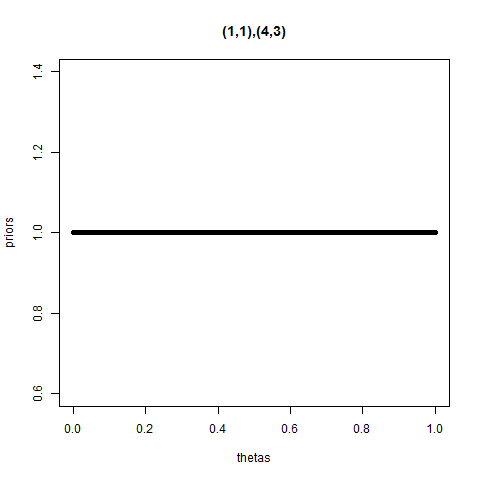
\includegraphics[width=5cm]{1143_prior2.png}
 \label{fig:boat1}
\end{multicols}

\begin{multicols}{2}
Posterior Distribution: 
\begin{align*}
    g(\theta | n,k) &= \frac{\Gamma (n+r+s)}{\Gamma (r+k) \Gamma (n-k+s)} \\
    & \cdot \theta^{r+k-1}(1-\theta)^{n+s-k-1} \\
    g(\theta | n,k) &= \frac{\Gamma (6)}{\Gamma (4) \Gamma (2)} \theta^{3}(1-\theta)^{1} \\
    g(\theta | n,k) &= \frac{6!}{4!8!} \theta^{3}(1-\theta)^{1} \\
    g(\theta | n,k) &= 15 \cdot \theta^{3}(1-\theta)^{1} \\
\end{align*}
\columnbreak
  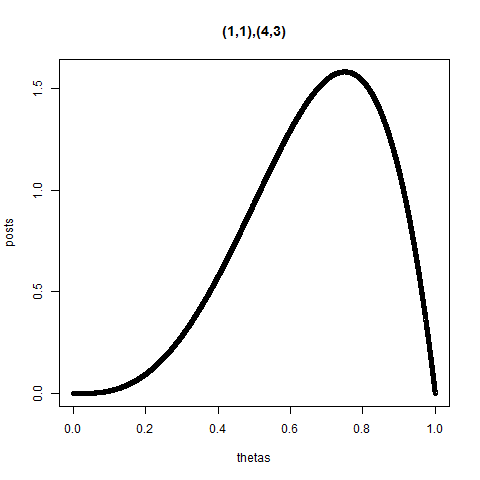
\includegraphics[width=5cm]{1143_post.png}
 \label{fig:boat1}
\end{multicols}

To find the probability of bias: $P(\theta > 0.5) = \int_{0.5}^{\infty} g(\theta ) d\theta =  1/2$\footnote{Could not figure out how to do this in R so I used wolfram alpha. I still don't really get it though. Because it only lets me do 2 parameters not 4.} 

\end{problem}
\newpage
%%%%%%%%%%%%%%%%%%%%%%%%%%%%%%%%%%%%%%%%%%%%%%%%%%%%%%%%
%%%%%%%%%%%%%%%%%%%%%%%%%%%%%%%%%%%%%%%%%%%%%%%%%%%%%%%%
%%%%%%%%%%%%%%%%%%%%%%%%%%%%%%%%%%%%%%%%%%%%%%%%%%%%%%%%

\begin{problem}{(1,1),(20,11)}.
\begin{multicols}{2}
 Prior Distribution: 
\begin{align*}
  g(\theta) &= \frac{\Gamma (r+s)}{\Gamma (r) \Gamma (s)} \theta^{r-1}(1-\theta)^{s-1} \\
    g(\theta) &= \frac{\Gamma (2)}{2\Gamma (1)} \theta^{0}(1-\theta)^{0} \\
    g(\theta) &= 1 
\end{align*}
\columnbreak
  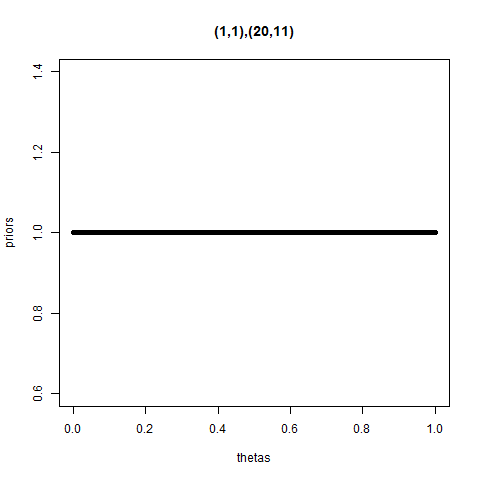
\includegraphics[width=5cm]{112011_prior2.png}
 \label{fig:boat1}
\end{multicols}

\begin{multicols}{2}
Posterior Distribution: 
\begin{align*}
    g(\theta | n,k) &= \frac{\Gamma (n+r+s)}{\Gamma (r+k) \Gamma (n-k+s)} \\
    & \cdot \theta^{r+k-1}(1-\theta)^{n+s-k-1} \\
    g(\theta | n,k) &= \frac{\Gamma (22)}{\Gamma (12) \Gamma (10)} \theta^{11}(1-\theta)^{9} \\
    g(\theta | n,k) &= \frac{22!}{12!32!} \theta^{11}(1-\theta)^{9} \\
    g(\theta | n,k) &= 646646 \cdot \theta^{11}(1-\theta)^{9} \\
\end{align*}
\columnbreak
  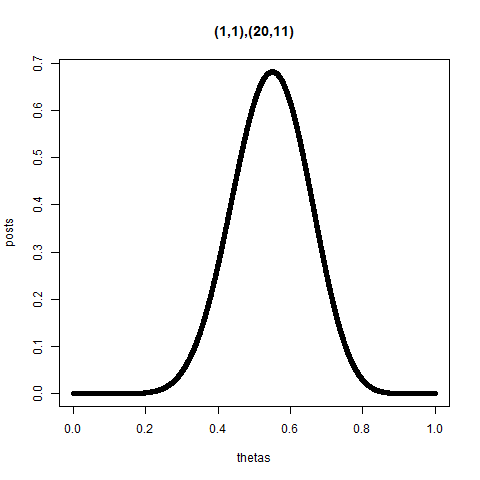
\includegraphics[width=5cm]{112011_post.png}
 \label{fig:boat1}
\end{multicols}
To find the probability of bias: $P(\theta > 0.5) = \int_{0.5}^{\infty} g(\theta ) d\theta =  1/2$

\end{problem}
\newpage
%%%%%%%%%%%%%%%%%%%%%%%%%%%%%%%%%%%%%%%%%%%%%%%%%%%%%%%%
%%%%%%%%%%%%%%%%%%%%%%%%%%%%%%%%%%%%%%%%%%%%%%%%%%%%%%%%
\begin{problem}{(4,4),(4,3)}.
\begin{multicols}{2}
 Prior Distribution: 
\begin{align*}
  g(\theta) &= \frac{\Gamma (r+s)}{\Gamma (r) \Gamma (s)} \theta^{r-1}(1-\theta)^{s-1} \\
    g(\theta) &= \frac{\Gamma (8)}{2\Gamma (4)} \theta^{3}(1-\theta)^{3} \\
    g(\theta) &= 840 \cdot \theta^{3}(1-\theta)^{3}
\end{align*}
\columnbreak
  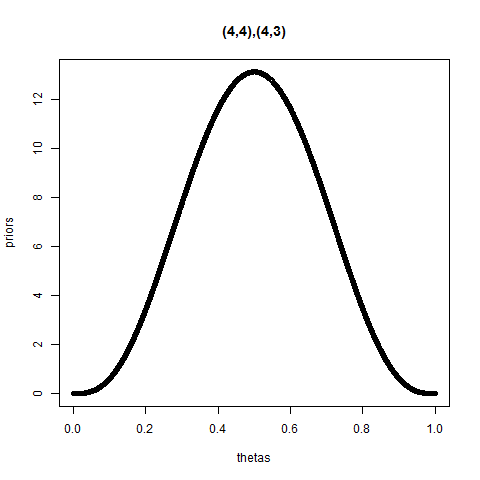
\includegraphics[width=5cm]{4443_prior2.png}
 \label{fig:boat1}
\end{multicols}

\begin{multicols}{2}
Posterior Distribution: 
\begin{align*}
    g(\theta | n,k) &= \frac{\Gamma (n+r+s)}{\Gamma (r+k) \Gamma (n-k+s)} \\
    & \cdot \theta^{r+k-1}(1-\theta)^{n+s-k-1} \\
    g(\theta | n,k) &= \frac{\Gamma (12)}{\Gamma (7) \Gamma (5)} \theta^{6}(1-\theta)^{3} \\
    g(\theta | n,k) &= \frac{12!}{7!11!} \theta^{6}(1-\theta)^{3} \\
    g(\theta | n,k) &= 792 \cdot \theta^{6}(1-\theta)^{3} \\
\end{align*}
\columnbreak
  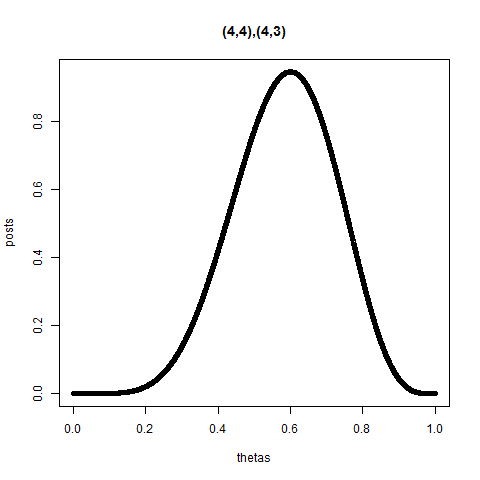
\includegraphics[width=5cm]{4443_post.png}
 \label{fig:boat1}
\end{multicols}
To find the probability of bias: $P(\theta > 0.5) = \int_{0.5}^{\infty} g(\theta ) d\theta =  0.5785$

\end{problem}
\newpage
%%%%%%%%%%%%%%%%%%%%%%%%%%%%%%%%%%%%%%%%%%%%%%%%%%%%%%%%
%%%%%%%%%%%%%%%%%%%%%%%%%%%%%%%%%%%%%%%%%%%%%%%%%%%%%%%%

\begin{problem}{(4,4),(20,11)}.
\begin{multicols}{2}
 Prior Distribution: 
\begin{align*}
  g(\theta) &= \frac{\Gamma (r+s)}{\Gamma (r) \Gamma (s)} \theta^{r-1}(1-\theta)^{s-1} \\
    g(\theta) &= \frac{\Gamma (8)}{2\Gamma (4)} \theta^{3}(1-\theta)^{3} \\
    g(\theta) &= 840 \cdot \theta^{3}(1-\theta)^{3}
\end{align*}
\columnbreak
  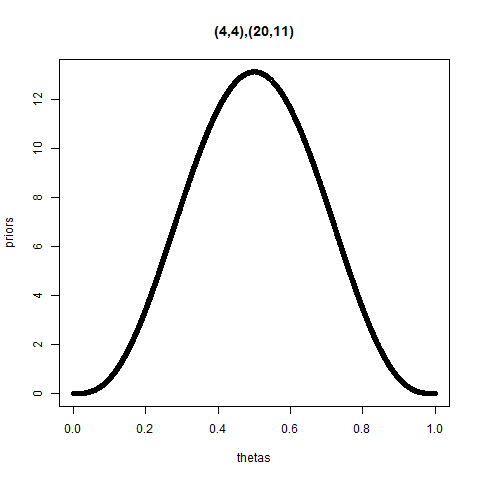
\includegraphics[width=5cm]{442011_prior2.png}
 \label{fig:boat1}
\end{multicols}

\begin{multicols}{2}
Posterior Distribution: 
\begin{align*}
    g(\theta | n,k) &= \frac{\Gamma (n+r+s)}{\Gamma (r+k) \Gamma (n-k+s)} \\
    & \cdot \theta^{r+k-1}(1-\theta)^{n+s-k-1} \\
    g(\theta | n,k) &= \frac{\Gamma (28)}{\Gamma (15) \Gamma (13)} \theta^{14}(1-\theta)^{12} \\
    g(\theta | n,k) &= \frac{28!}{15!13!} \theta^{14}(1-\theta)^{12} \\
    g(\theta | n,k) &= 37442160 \cdot \theta^{14}(1-\theta)^{12} \\
\end{align*}
\columnbreak
  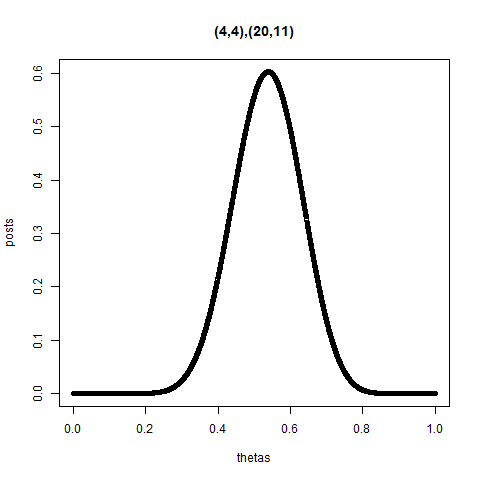
\includegraphics[width=5cm]{442011_post.png}
 \label{fig:boat1}
\end{multicols}

To find the probability of bias: $P(\theta > 0.5) = \int_{0.5}^{\infty} g(\theta ) d\theta =  0.648$

\end{problem}
\newpage

\end{document}


